\documentclass{article}
\usepackage[spanish]{babel}
\usepackage[utf8]{inputenc}
\usepackage[T1]{fontenc}
\usepackage{titlesec}
\usepackage{hyperref}
\usepackage{graphicx}
\usepackage{caption}
\usepackage{subcaption}
\usepackage{fancyhdr}
\usepackage[document]{ragged2e}
\pagestyle{fancy}
    \fancyhf{}
    \fancyfoot[C]{\thepage}
    \fancyfoot[L]{\ifodd\value{page}\textit{\small Gu\'ia de estudio Mapas de Calor }\else\textit{\small Carlos E Martínez-Rodríguez}\fi}
    \fancyfoot[R]{\ifodd\value{page}\textit{\small Carlos E Martínez-Rodríguez}\else\textit{\small Gu\'ia de estudio Mapa de Calor }\fi}
\usepackage[left=2cm,right=2cm,top=2cm,bottom=2cm]{geometry}
\renewcommand{\sectionmark}[1]{\markright{#1}}
\fancyhead[LE,RO]{\nouppercase{\rightmark}}
\fancyhead[LO,RE]{\nouppercase{\leftmark}}
% << == >>  << == >>  << == >>  << == >>  << == >>  << == >>  << == >>  << == >>  << 
% Título y autor del documento
\title{An\'alisis de Cl\'usters, Componentes Principales y Mapas de Calor}
\author{Carlos E Martinez-Rodriguez}
% << == >>  << == >>  << == >>  << == >>  << == >>  << == >>  << == >>  << == >>  << 
\begin{document}
% ==============================================================
\maketitle
\tableofcontents
\medskip
% ===============================================================

\section{Introducción}

Un mapa de calor es una representación gráfica en la que los valores de una matriz se muestran mediante colores. Cada celda de la matriz se asigna a un color según su valor, lo que permite visualizar fácilmente las variaciones, distribuci\'on e intensidad de una variable en una matriz de datos. Los mapas de calor son especialmente útiles cuando se trabaja con matrices de datos grandes y multidimensionales, adem\'as de que  permiten visualizar patrones, tendencias y variaciones en los datos de manera efectiva.\medskip

 La principal ventaja de los mapas de calor es su capacidad para resaltar las diferencias relativas entre los valores en una matriz. Al asignar colores a los valores, los mapas de calor permiten una fácil identificación de las regiones con valores altos o bajos en comparación con el resto de la matriz. \medskip
 
Además, los mapas de calor permiten visualizar relaciones y patrones entre filas y columnas de la matriz. Al ordenar las filas y columnas según alguna métrica (por ejemplo, mediante agrupación jerárquica o clasificación), se pueden identificar agrupaciones y similitudes entre elementos. Esto facilita la identificación de clústeres, tendencias o relaciones entre diferentes variables o muestras.


% - - - - - - - -   - - - - - - - -   - - - - - - - -   - - - - - - - -   - - - - - - - - - - - - - - - - 
\subsection{Utilidad de los mapas de calor en la visualización de datos}
Los mapas de calor son especialmente útiles cuando se trabaja con conjuntos de datos grandes y multidimensionales. Algunas de las aplicaciones comunes de los mapas de calor en la visualización de datos incluyen:

\begin{itemize}
    \item Identificación de patrones y tendencias en datos climáticos y meteorológicos.
    \item Análisis de la distribución de la temperatura en imágenes térmicas.
    \item Visualización de datos de rendimiento en deportes para identificar fortalezas y debilidades.
    \item Análisis de expresión génica en biología molecular para identificar genes activos o inactivos.
    \item Representación de datos de mercado y finanzas para identificar áreas de crecimiento o declive.
\end{itemize}

% - - - - - - - -   - - - - - - - -   - - - - - - - -   - - - - - - - -   - - - - - - - - - - - - - - - - 
\subsection{Construcción de mapas de calor}

Existen varias técnicas y herramientas para construir mapas de calor. En R, existen varias bibliotecas populares para generar mapas de calor. Algunas de las librerías más utilizadas son:

\begin{itemize}
\item \textbf{ggplot2}: Es una de las bibliotecas más populares y versátiles en R para visualización de datos. Si bien no es específicamente una biblioteca para mapas de calor, se puede utilizar para crear mapas de calor utilizando la función \texttt{geom-tile()} para representar los valores de los datos como colores en una cuadrícula.

\item \textbf{heatmap}: Es una biblioteca base de R que proporciona funciones para generar mapas de calor. La función \texttt{heatmap()} crea un mapa de calor basado en una matriz de datos numéricos, donde los valores son representados por colores.

\item \textbf{heatmaply}: Esta biblioteca utiliza la biblioteca plotly para generar mapas de calor interactivos en R. Proporciona funciones para crear mapas de calor 2D y 3D, y permite explorar los mapas de calor con características interactivas como zoom, rotación y selección de puntos.

\item \textbf{pheatmap}: Es una biblioteca especializada en la generación de mapas de calor en R. Proporciona una amplia gama de opciones de personalización, como la configuración de colores, el ordenamiento de filas y columnas, y la adición de anotaciones a los mapas de calor.

\item \textbf{ComplexHeatmap}: Es una biblioteca avanzada para la generación de mapas de calor complejos en R. Permite crear mapas de calor con múltiples capas de información, como anotaciones, dendrogramas y matrices de distancias.
\end{itemize}


% - - - - - - - -   - - - - - - - -   - - - - - - - -   - - - - - - - -   - - - - - - - - - - - - - - - - 
\subsection{Personalización de los mapas de calor}
Los mapas de calor se pueden personalizar para adaptarse a las necesidades específicas de los datos y la visualización. Algunas de las opciones de personalización incluyen:

\begin{itemize}
\item  \textbf{Selección de colores: }es posible elegir una paleta de colores adecuada para resaltar las variaciones en los datos. La elección de colores es esencial para la interpretación adecuada de los mapas de calor. R ofrece varias paletas de colores predefinidas, pero también es posible definir colores personalizados.

\item  \textbf{Escalas de color: }se pueden ajustar las escalas de color para resaltar áreas de alta o baja intensidad. La selección de escalas es un paso crítico en la construcción de mapas de calor. En general, existen dos tipos de escalas comúnmente utilizadas: escalas lineales y escalas logarítmicas. La elección de la escala depende de la naturaleza de los datos y del objetivo del análisis. Si los datos abarcan un rango amplio y se desea resaltar las diferencias en valores pequeños, es recomendable utilizar una escala logarítmica. Por otro lado, si los datos se distribuyen de manera más uniforme, una escala lineal puede ser más adecuada.


En este ejemplo, se utiliza la función `colorRampPalette` para definir una paleta de colores que va desde el azul hasta el rojo. Esta paleta personalizada se pasa como argumento a la función `heatmap` para construir el mapa de calor.

Además de los colores, es importante seleccionar la escala adecuada para los mapas de calor. R ofrece varias opciones de escalas, como escalas lineales y logarítmicas. A continuación se muestra un ejemplo de cómo seleccionar una escala para un mapa de calor en R:

\begin{verbatim}
# Cargar la librería pheatmap
library(pheatmap)

# Crear una matriz de ejemplo
matriz <- matrix(rnorm(100), nrow = 10)

# Construir el mapa de calor utilizando una escala logarítmica
pheatmap(matriz, scale = "log")
\end{verbatim}

En este ejemplo, se utiliza la función `pheatmap` de la librería pheatmap para construir el mapa de calor. El argumento `scale` se establece en "log" para utilizar una escala logarítmica en el mapa de calor.

    
    \item Anotaciones y etiquetas: es posible agregar etiquetas y anotaciones a las celdas del mapa de calor para proporcionar información adicional.  Las anotaciones pueden proporcionar información adicional en los mapas de calor, como etiquetas de fila y columna, valores numéricos o etiquetas personalizadas. A continuación se muestra un ejemplo de cómo agregar anotaciones a un mapa de calor en R:

\begin{verbatim}
# Cargar la librería ComplexHeatmap
library(ComplexHeatmap)

# Crear una matriz de ejemplo
matriz <- matrix(rnorm(100), nrow = 10)

# Construir el mapa de calor con anotaciones de fila y columna
Heatmap(matriz, name = "Valor", row_names_side = "left", column_names_side = "top")
\end{verbatim}

En este ejemplo, se utiliza la función `Heatmap` de la librería ComplexHeatmap para construir el mapa de calor. Los argumentos `row\_names\_side` y `column\_names\_side` se establecen en "left" y "top", respectivamente, para agregar etiquetas de fila a la izquierda y etiquetas de columna en la parte superior del mapa de calor.

\begin{verbatim}
# Cargar la librería heatmap
library(heatmap)

# Crear una matriz de ejemplo
matriz <- matrix(rnorm(100), nrow = 10)

# Definir una paleta de colores personalizada
mi_paleta <- colorRampPalette(c("blue", "white", "red"))

# Construir el mapa de calor utilizando la paleta de colores personalizada
heatmap(matriz, col = mi_paleta)
\end{verbatim}

\end{itemize}

% - - - - - - - -   - - - - - - - -   - - - - - - - -   - - - - - - - -   - - - - - - - - - - - - - - - - 
\subsection{Interpretación de los mapas de calor}
La interpretación de los mapas de calor es crucial para comprender la distribución de los datos.  La interpretación de los mapas de calor se basa en la capacidad para percibir y distinguir diferentes colores.  Algunos aspectos a considerar al interpretar los mapas de calor son:

\begin{itemize}
\item Atención a la intensidad de los colores: los colores más intensos indican valores más altos o significativos, mientras que los colores más claros indican valores más bajos. Al utilizar una paleta de colores bien elegida, se pueden resaltar las diferencias y patrones de manera efectiva. Por ejemplo, se puede utilizar una paleta de colores divergente que resalte los valores extremos o una paleta de colores secuencial que muestre una progresión gradual de valores. La elección de la paleta de colores adecuada es crucial para garantizar una interpretación precisa y no sesgada de los datos.
\item Identificación de patrones y tendencias: buscar áreas de concentración o dispersión en el mapa de calor para identificar patrones y tendencias en los datos.
\item Comparación entre mapas de calor: comparar diferentes mapas de calor para identificar diferencias o similitudes en la distribución de la variable en diferentes conjuntos de datos.


\end{itemize}


% <><> <><> <><> <><> <><> <><> <><> <><> <><> <><> <><> <><> <><> <><> 
%\section{Construcción de mapas de calor}
% <><> <><> <><> <><> <><> <><> <><> <><> <><> <><> <><> <><> <><> <><>

% - - - - - - - -   - - - - - - - -   - - - - - - - -   - - - - - - - -   - - - - - - - - - - - - - - - - 
% - - - - - - - -   - - - - - - - -   - - - - - - - -   - - - - - - - -   - - - - - - - - - - - - - - - - 
\subsection{Preparación de datos}
Antes de construir un mapa de calor en R, es importante preparar los datos adecuadamente.  Es preciso asegurarse de tener una matriz o un dataframe con los datos que deseas visualizar, además de que los datos estén en el formato correcto y que no falten valores.  Preparación de los datos: Antes de construir un mapa de calor, es necesario realizar una preparación adecuada de los datos. Esto implica asegurarse de que los datos estén en el formato correcto y sean apropiados para su visualización en un mapa de calor. Si los datos están en forma de una matriz, es importante verificar que estén completos, es decir, no deben haber valores faltantes. En caso de que existan valores faltantes, es necesario tomar decisiones sobre cómo manejarlos, ya sea eliminando las filas o columnas correspondientes o imputando valores apropiados.

\subsection{Normalizaci\'on de los datos}
Antes de construir un mapa de calor, es común aplicar técnicas de normalización a los datos. La normalización tiene como objetivo ajustar los valores de los datos a una escala específica y facilitar la comparación entre diferentes elementos. En el caso de los mapas de calor, se utilizan dos enfoques de normalización comunes: normalización por filas y normalización por columnas.

En la normalización por filas, los valores de cada fila se escalan para que tengan una suma de 1 o una media de 0. Esto permite comparar la contribución relativa de cada valor dentro de una fila y resalta los patrones de distribución entre filas.

En la normalización por columnas, los valores de cada columna se escalan para que tengan una suma de 1 o una media de 0. Esto permite comparar la contribución relativa de cada valor dentro de una columna y resalta los patrones de distribución entre columnas.

% - - - - - - - -   - - - - - - - -   - - - - - - - -   - - - - - - - -   - - - - - - - - - - - - - - - - 
\subsection{Generaci\'on del mapa de calor}
Generación del mapa de calor: Una vez que los datos han sido preparados y normalizados, se procede a la construcción del mapa de calor. Esto implica asignar colores a los valores de la matriz normalizada y representarlos visualmente en una cuadrícula. La elección de la paleta de colores es importante para una interpretación adecuada del mapa de calor. Se deben seleccionar colores que sean perceptualmente distintos y que permitan una fácil identificación de los valores altos y bajos.

\subsubsection{Construcción de un mapa de calor básico con la librería heatmap}
A continuación se muestra un ejemplo de cómo construir un mapa de calor básico utilizando la librería heatmap en R:

\begin{verbatim}
# Cargar la librería heatmap
library(heatmap)

# Crear una matriz de ejemplo
matriz <- matrix(rnorm(100), nrow = 10)

# Construir el mapa de calor
heatmap(matriz)
\end{verbatim}

Este código generará un mapa de calor básico utilizando la función \texttt{heatmap} de la librería heatmap.  Es posible ajustar los parámetros de la función según lass necesidades, como los colores utilizados, la escala, entre otros.

% - - - - - - - -   - - - - - - - -   - - - - - - - -   - - - - - - - -   - - - - - - - - - - - - - - - - 
\subsubsection{Construcción de un mapa de calor con la librería ggplot2}

Para construir un mapa de calor más personalizable y estéticamente agradable, puedes utilizar la librería ggplot2. A continuación se muestra un ejemplo de cómo construir un mapa de calor utilizando la librería ggplot2:

\begin{verbatim}
# Cargar la librería ggplot2
library(ggplot2)

# Crear una matriz de ejemplo
matriz <- matrix(rnorm(100), nrow = 10)

# Convertir la matriz a un dataframe
df <- as.data.frame(matriz)

# Construir el mapa de calor utilizando ggplot2
ggplot(df, aes(x = factor(1), y = factor(1), fill = V1)) +
  geom_tile() +
  scale_fill_gradient(low = "blue", high = "red") +
  theme_void()
\end{verbatim}

Este código generará un mapa de calor utilizando la función \texttt{ggplot} de la librería ggplot2. Puedes personalizar el mapa de calor ajustando los parámetros de la función, como los colores utilizados, la escala, entre otros.



\section{An\'alisis alternativo}

El análisis de clusters es una técnica fundamental en Bioinformática que permite agrupar objetos similares en conjuntos homogéneos. En el contexto de la investigación genómica y proteómica, el análisis de clusters se utiliza para identificar patrones, descubrir relaciones entre genes o proteínas, y clasificar muestras en función de su perfil molecular. Este enfoque juega un papel crucial en la comprensión de la estructura y función de los datos biológicos, así como en la identificación de biomarcadores y el descubrimiento de nuevas terapias. 

El análisis de clusters  consiste en agrupar objetos similares en conjuntos homogéneos, donde la similitud se basa en medidas específicas según el tipo de datos (por ejemplo, distancias genéticas, correlaciones de expresión génica o similitud de secuencias). El análisis de clusters es esencial en Bioinformática por varias razones:

\begin{enumerate}
\item Descubrimiento de patrones y relaciones: Permite identificar grupos de genes o proteínas con perfiles de expresión similares, lo que sugiere su función común en procesos biológicos específicos. Además, puede ayudar a descubrir relaciones entre diferentes muestras, como en el caso de la clasificación de pacientes en subtipos de enfermedades o en la identificación de especies relacionadas.
\item Identificación de biomarcadores: Los biomarcadores son características moleculares que se asocian con enfermedades, estados patológicos o respuestas a tratamientos. El análisis de clusters puede revelar patrones moleculares distintivos en diferentes grupos de pacientes, lo que ayuda a identificar biomarcadores potenciales para el diagnóstico, pronóstico y selección de terapias personalizadas.

\item Visualización de datos: Los resultados del análisis de clusters se pueden representar gráficamente mediante dendrogramas, mapas de calor u otras visualizaciones, lo que facilita la interpretación y comunicación de los patrones encontrados. Estas representaciones visuales permiten una comprensión más intuitiva de los datos y pueden guiar investigaciones posteriores.

\item Agrupamiento de secuencias biológicas: En el campo de la genómica y la proteómica, el análisis de clusters es esencial para agrupar secuencias de ADN, ARN o proteínas similares. Esto facilita la identificación de familias de genes o proteínas relacionadas, así como la predicción de funciones basadas en la similitud de secuencias.

\item Exploración de datos de alto rendimiento: Con la creciente disponibilidad de conjuntos de datos de alto rendimiento, como los datos de secuenciación masiva o los perfiles de expresión a gran escala, el análisis de clusters se ha convertido en una herramienta imprescindible. Permite analizar grandes volúmenes de datos de manera eficiente y extraer información valiosa de ellos.
\end{enumerate}


\subsection{Teoría matemática de los mapas de calor}

Los mapas de calor son una representación visual utilizada para mostrar la distribución y la intensidad de los valores en una matriz de datos. Esta representación se basa en la asignación de colores a los valores numéricos, donde los colores más claros indican valores altos y los colores más oscuros indican valores bajos. La teoría matemática detrás de los mapas de calor involucra los siguientes conceptos:

\begin{itemize}
% ----------------------------------------------------------------------------------------------------------------
\item \textbf{Normalización: } Antes de generar un mapa de calor, es común realizar una normalización de los datos. La normalización tiene como objetivo escalar los valores de la matriz de datos a un rango común, lo que permite una comparación más precisa entre los valores. Una técnica común de normalización es la normalización por filas o por columnas, donde se calcula el valor relativo de cada dato con respecto a los demás en la misma fila o columna.
\begin{itemize}
\item \textbf{Normalización por filas:}
Dada una matriz de datos  $X$ de tamaño  $m \times n$,  la normalización por filas se realiza calculando el valor relativo de cada dato con respecto a los demás en la misma fila. Para cada elemento  $x_{ij}$ de la matriz, la normalización por filas se calcula de la siguiente manera: $$x_{ij}^{'} = \frac{x_{ij}}{\sqrt{\sum_{k=1}^{n} x_{ik}^2}}$$

Este enfoque permite resaltar los patrones de variación dentro de cada renglón. 

\item \textbf{Normalización por columnas:}
Dada una matriz de datos  $X$ de tamaño  $m \times n$,   la normalización por columnas se realiza calculando el valor relativo de cada dato con respecto a los demás en la misma columna. Para cada elemento  $x_{ij}$  de la matriz, la normalización por columnas se calcula de la siguiente manera:$$x_{ij}^{'} = \frac{x_{ij}}{\sqrt{\sum_{k=1}^{m} x_{kj}^2}}$$.

En ambas fórmulas, $x_{ij}^{'}$ representa el valor normalizado del elemento $x_{ij}$, $\sum_{k=1}^{n} x_{ik}^2$ es la suma de los cuadrados de los elementos en la misma fila y $\sum_{k=1}^{m} x_{kj}^2$ es la suma de los cuadrados de los elementos en la misma columna. La normalización por filas y por columnas asegura que los valores en cada fila o columna tengan una magnitud comparable y permite una comparación más precisa entre los valores de la matriz de datos.

\end{itemize}

La normalización de datos es esencial para asegurar que los mapas de calor reflejen de manera precisa los patrones y relaciones presentes en los datos originales. Los mapas de calor normalizados permiten una visualización más efectiva y facilitan la identificación de las regiones con mayores y menores valores en la matriz de datos.



% --------------------------------------------------------------------------------
\item\textbf{Colormap: } La colormap es una función que asigna valores numéricos a colores. Define la correspondencia entre los valores de los datos y los colores que se mostrarán en el mapa de calor. Existen diversas colormaps disponibles, como el mapa de colores \textit{jet}, \textit{hot}, \textit{cool}, entre otros. Cada colormap tiene una gama de colores que van desde un color inicial (por ejemplo, azul) hasta un color final (por ejemplo, rojo) que representan los valores mínimos y máximos de la escala.


La función de asignación en una colormap define la correspondencia entre los valores numéricos de los datos y los colores que se mostrarán en el mapa de calor.  Dada una colormap, se utiliza una función que mapea un valor numérico a un color específico en la escala de colores. La función de asignación toma como entrada un valor numérico y devuelve el color correspondiente según la escala establecida en la colormap. 

En una colormap, los valores numéricos de los datos se asignan a colores específicos siguiendo una escala de colores predefinida. Por ejemplo, en la colormap \textit{jet}, los valores mínimos se representan con colores más fríos como el azul, mientras que los valores máximos se representan con colores más cálidos como el rojo. La función de asignación mapea los valores numéricos en la escala de los valores mínimos y máximos definidos en la colormap, asignando colores correspondientes a cada valor.

Cabe mencionar que existen diversas colormaps disponibles, cada una con una gama de colores específica y una asignación única de valores numéricos a colores. Algunas colormaps comunes incluyen \textit{jet}, \textit{hot}, \textit{cool}, entre otras. La elección de la colormap adecuada depende del tipo de datos y la representación visual deseada.

\begin{equation}
\textrm{{color}} = f(\textrm{{valor}})
\end{equation}

Donde "color" representa el valor de color asignado y "valor" es el valor numérico al que se le asigna el color. La función $f$ define la correspondencia específica entre el valor numérico y el color correspondiente en la escala de colores. Esta función puede variar dependiendo de la colormap utilizada y cómo se defina la escala de colores.
\begin{itemize}
\item \textbf{Asignación lineal:}
\begin{equation}
\textrm{{color}} = m \cdot \textrm{{valor}} + b
\end{equation}
Esta función asigna colores de manera lineal, donde $m$ y $b$ son constantes que determinan la pendiente y el desplazamiento de la línea.

\item \textbf{Asignación logarítmica:}
\begin{equation}
\textrm{{color}} = a \cdot \log(\textrm{{valor}}) + b
\end{equation}
Esta función asigna colores utilizando una escala logarítmica, donde $a$ y $b$ son constantes que afectan la amplitud y el desplazamiento de la función logarítmica.

\item \textbf{Asignación exponencial:}
\begin{equation}
\textrm{{color}} = a \cdot \exp(b \cdot \textrm{{valor}})
\end{equation}
Esta función asigna colores utilizando una escala exponencial, donde $a$ y $b$ son constantes que controlan la amplitud y la tasa de crecimiento exponencial.

\end{itemize}

% ----------------------------------------------------------------------------------------------------------------
\item\textbf{Interpolación: } La interpolación se utiliza para asignar colores a los valores que no están representados explícitamente en la matriz de datos. La interpolación se realiza mediante algoritmos que estiman los valores entre los puntos de datos conocidos. Por ejemplo, si hay una celda vacía en la matriz de datos, se puede utilizar la interpolación para estimar el valor correspondiente y asignarle un color en el mapa de calor.

La interpolación es una técnica utilizada para estimar valores intermedios entre puntos de datos conocidos. En el contexto de asignar colores a los valores en un mapa de calor, la interpolación se utiliza cuando hay celdas vacías o valores faltantes en la matriz de datos. La interpolación nos permite estimar esos valores faltantes y asignarles un color correspondiente.

Una forma común de realizar la interpolación en este caso es utilizar



\begin{itemize}
\item  \textbf{Interpolación lineal: }Supongamos que tenemos un conjunto de puntos de datos conocidos $(x_1, y_1)$, $(x_2, y_2)$, $\ldots$,$ (x_n, y_n)$, donde $x_i$ representa la posición en el eje $x$ y $y_i$ es el valor asociado en ese punto. Queremos estimar el valor $y$ en un punto intermedio $x$ que no está explícitamente representado en la matriz de datos.

La interpolación lineal se basa en la idea de que el cambio en los valores $y$ es proporcional al cambio en los valores $x$ entre los puntos conocidos. La fórmula de interpolación lineal se puede expresar matemáticamente como:

\begin{equation}
y = y_i + \frac{{(x - x_i)}}{{(x_{i+1} - x_i)}} \cdot (y_{i+1} - y_i)
\end{equation}

donde $x_i$ y $x_{i+1}$ son los puntos de datos conocidos más cercanos al punto intermedio $x$, y $y_i$ y $y_{i+1}$ son los valores correspondientes asociados a esos puntos.

Utilizando esta fórmula de interpolación lineal, podemos estimar el valor faltante en la matriz de datos y asignarle un color en el mapa de calor. La interpolación nos permite obtener una representación visual más completa de los datos, rellenando las celdas vacías con valores estimados basados en la información disponible en los puntos conocidos.

\item   \textbf{Interpolación polinómica:}
La interpolación polinómica es un método que utiliza polinomios para ajustar los puntos de datos conocidos y estimar los valores intermedios. Uno de los métodos más comunes es la interpolación de Lagrange. Dado un conjunto de puntos $(x_0, y_0), (x_1, y_1), \ldots, (x_n, y_n)$, donde $x_i$ son las abscisas y $y_i$ son las ordenadas de los puntos, el polinomio de Lagrange se define como:

\begin{equation}
    P(x) = \sum_{i=0}^{n} y_i \cdot \prod_{j=0, j \neq i}^{n} \frac{x - x_j}{x_i - x_j}
\end{equation}

Este polinomio pasa exactamente por todos los puntos conocidos y se utiliza para estimar los valores intermedios.

\item   \textbf{Interpolación spline:}

La interpolación spline utiliza funciones suaves llamadas splines para estimar los valores faltantes. Un spline es una curva definida en segmentos que se ajusta a los puntos de datos conocidos. En la interpolación spline cúbica, se utilizan polinomios de tercer grado para cada segmento. El spline cúbico se puede representar mediante ecuaciones polinómicas de la forma:

\begin{equation}
    S_i(x) = a_i + b_i(x - x_i) + c_i(x - x_i)^2 + d_i(x - x_i)^3 \quad \textrm{para } x_i \leq x \leq x_{i+1}
\end{equation}

donde $a_i$, $b_i$, $c_i$ y $d_i$ son coeficientes que se determinan utilizando condiciones de continuidad y suavidad en los puntos conocidos.

\item  \textbf{ Interpolación vecino más cercano:}

La interpolación vecino más cercano asigna el valor del punto de datos conocido más cercano al punto intermedio sin realizar cálculos adicionales. En esta técnica, el color asignado al punto intermedio será el mismo color que el punto conocido más cercano. Matemáticamente, se puede representar como:

\begin{equation}
    f(x) = f(x_{\textrm{vecino más cercano}})
\end{equation}

donde $f(x)$ es el valor estimado para el punto intermedio y $x_{\textrm{vecino más cercano}}$ es el punto de datos conocido más cercano a $x$.

\item   \textbf{Interpolación Kriging:}

El Kriging es un método avanzado que considera la estructura espacial y la correlación de los datos para realizar la interpolación. Se basa en modelos geoestadísticos y se utiliza principalmente en análisis espacial y geología. La estimación Kriging se calcula como una combinación lineal ponderada de los valores conocidos en función de su distancia y correlación espacial. La ecuación general del Kriging es:

\begin{equation}
    Z(x) = \sum_{i=1}^{n} \lambda_i Z(x_i)
\end{equation}

donde $Z(x)$ es el valor estimado para el punto intermedio, $Z(x_i)$ son los valores conocidos, $\lambda_i$ son los pesos asignados a cada valor conocido y $n$ es el número de puntos conocidos.
\end{itemize}

Estas son algunas de las funciones de interpolación utilizadas en la generación de mapas de calor.
% ----------------------------------------------------------------------------------------------------------------
\item\textbf{Escalado: } El escalado se utiliza para ajustar la intensidad de los colores en el mapa de calor. Permite resaltar o atenuar la diferencia de intensidad entre los valores para una mejor visualización. Se pueden utilizar diferentes métodos de escalado, como el escalado lineal, el escalado logarítmico o el escalado basado en percentiles, dependiendo de las características de los datos y el propósito de la representación.

\begin{itemize}
\item   \textbf{Escalado lineal:}

El escalado lineal es el método más simple y directo de escalado. Consiste en ajustar los valores de los datos a un rango específico, generalmente entre 0 y 1 o entre un valor mínimo y máximo predefinidos. La fórmula para el escalado lineal es:

\begin{equation}
    \textrm{valor escalado} = \frac{\textrm{valor original} - \textrm{mínimo}}{\textrm{máximo} - \textrm{mínimo}}
\end{equation}

El escalado lineal preserva la proporción de las diferencias entre los valores originales, pero puede verse afectado por valores atípicos y puede no resaltar adecuadamente las diferencias entre valores cercanos.

\item   \textbf{Escalado logarítmico:}

El escalado logarítmico se utiliza cuando los datos abarcan un rango muy amplio y se desea resaltar las diferencias en los valores más pequeños. El escalado logarítmico aplica una transformación logarítmica a los datos antes de realizar el escalado lineal. La fórmula para el escalado logarítmico es:

\begin{equation}
    \textrm{valor escalado} = \frac{\log(\textrm{valor original} - \textrm{mínimo} + 1)}{\log(\textrm{máximo} - \textrm{mínimo} + 1)}
\end{equation}

El escalado logarítmico comprime los valores más grandes y expande los valores más pequeños, lo que puede revelar mejor las diferencias en la parte inferior de la escala. Sin embargo, es importante tener en cuenta que no se puede aplicar a valores negativos o cero.

\item   \textbf{Escalado basado en percentiles:}

El escalado basado en percentiles se utiliza cuando se desea resaltar las diferencias en ciertos rangos de valores. En este método, los valores se escalan en función de sus posiciones relativas dentro de la distribución. Por ejemplo, se puede asignar el percentil 5 al valor mínimo y el percentil 95 al valor máximo. La fórmula para el escalado basado en percentiles es:

\begin{equation}
    \textrm{valor escalado} = \frac{\textrm{rango percentil del valor original} - \textrm{percentil mínimo}}{\textrm{percentil máximo} - \textrm{percentil mínimo}}
\end{equation}

El escalado basado en percentiles resalta las diferencias en ciertos rangos de valores, lo que puede ser útil para destacar valores atípicos o concentraciones de datos en áreas específicas.
\end{itemize}


\item \textbf{Eliminacion de datos faltantes: }
En el análisis de datos, es común enfrentarse a valores faltantes o datos ausentes en el conjunto de datos. Estos valores pueden ser el resultado de diversas circunstancias, como errores de medición, pérdida de datos durante la recolección o problemas técnicos.

En el caso específico de los mapas de calor, la presencia de datos faltantes puede afectar la precisión y la interpretación de los resultados. 

\begin{itemize}
\item   \textbf{Preservar la coherencia visual: }Los mapas de calor se utilizan para visualizar patrones y relaciones en los datos, y se basan en la comparación de los valores numéricos. Cuando se eliminan los datos faltantes, se asegura que los patrones y las relaciones sean consistentes y no se distorsionen debido a los valores ausentes. Esto permite una interpretación más precisa de los resultados.

\item   \textbf{Facilitar el análisis y la interpretación: }Los datos faltantes pueden introducir incertidumbre y complejidad en el análisis de los datos. Al eliminar los datos faltantes, se simplifica el conjunto de datos y se facilita su análisis y la interpretación de los resultados. Los patrones emergentes se vuelven más evidentes y se reduce la posibilidad de conclusiones erróneas debido a los valores ausentes.

\item   \textbf{Evitar sesgos en los resultados: }La presencia de datos faltantes puede introducir sesgos en el análisis de datos y en los resultados obtenidos. Dependiendo de la naturaleza de los datos faltantes, pueden existir sesgos sistemáticos en ciertas variables o subconjuntos de datos. Al eliminar los datos faltantes, se minimiza la posibilidad de sesgos y se promueve la imparcialidad en el análisis.
\end{itemize}

Sin embargo, es importante destacar que la eliminación de datos faltantes debe realizarse con cuidado y considerando el contexto específico del análisis. Algunas consideraciones adicionales son:

\begin{itemize}
\item   \textbf{Evaluar el patrón de los datos faltantes: }Es importante examinar si los datos faltantes siguen un patrón específico, como datos faltantes aleatorios o datos faltantes sistemáticos. Esto puede influir en la decisión de eliminar o imputar los valores faltantes.

\item   \textbf{Evaluar el impacto en el tamaño y la representatividad de la muestra: } Eliminar los datos faltantes puede reducir el tamaño de la muestra y afectar la representatividad de los datos. Es fundamental evaluar si la eliminación de los datos faltantes introduce algún sesgo en la muestra y si la muestra resultante sigue siendo adecuada para el análisis.

\item   \textbf{Considerar técnicas de imputación de datos: }En algunos casos, puede ser apropiado utilizar técnicas de imputación de datos para estimar los valores faltantes en lugar de eliminarlos por completo. Estas técnicas permiten preservar el tamaño de la muestra y proporcionar una aproximación de los valores ausentes. Sin embargo, es importante evaluar la idoneidad de las técnicas de imputación y los supuestos asociados.
\end{itemize}
% ----------------------------------------------------------------------------------------------------------------

\item\textbf{Generación del mapa de calor: } Una vez que se ha realizado la normalización de los datos, se ha definido la colormap y se han aplicado las técnicas de interpolación y escalado, se procede a generar el mapa de calor. Esto implica asignar colores a cada valor en la matriz de datos según la colormap y visualizar la matriz resultante en forma de una imagen o gráfico.

\begin{itemize}
\item   \textbf{Normalización de los datos:}

La normalización de los datos es un paso importante antes de generar el mapa de calor. El objetivo es escalar los valores de la matriz de datos a un rango común para permitir una comparación más precisa entre los valores. Una técnica común de normalización es la normalización por filas o por columnas. La fórmula para la normalización por filas es:

\begin{equation}
    \textrm{valor normalizado} = \frac{\textrm{valor original} - \textrm{valor mínimo en la fila/columna}}{\textrm{valor máximo en la fila/columna} - \textrm{valor mínimo en la fila/columna}}
\end{equation}

La normalización por columnas se realiza de manera similar, pero utilizando los valores mínimo y máximo en la columna correspondiente.

\item   \textbf{Definición de la colormap:}

La colormap es una función que asigna valores numéricos a colores. Define la correspondencia entre los valores de los datos y los colores que se mostrarán en el mapa de calor. Existen diversas colormaps disponibles, como el mapa de colores \textrm{jet}, \textrm{hot}, \textrm{cool}, entre otros. Cada colormap tiene una gama de colores que representa los valores mínimos y máximos de la escala. La asignación de valores a colores puede realizarse mediante una función específica que mapea los valores al espacio de color.

\item   \textbf{Aplicación de técnicas de interpolación y escalado:}

Después de la normalización y la definición de la colormap, se aplican técnicas de interpolación y escalado para asignar colores a cada valor en la matriz de datos. La interpolación se utiliza para asignar colores a los valores que no están representados explícitamente en la matriz de datos. Se utilizan algoritmos que estiman los valores entre los puntos de datos conocidos. Por ejemplo, si hay una celda vacía en la matriz de datos, se puede utilizar la interpolación para estimar el valor correspondiente y asignarle un color en el mapa de calor.

El escalado se utiliza para ajustar la intensidad de los colores en el mapa de calor, resaltando o atenuando la diferencia de intensidad entre los valores para una mejor visualización. Se pueden utilizar diferentes métodos de escalado, como el escalado lineal, el escalado logarítmico o el escalado basado en percentiles, dependiendo de las características de los datos y el propósito de la representación.

\item   \textbf{Generación del mapa de calor:}

Una vez que se ha realizado la normalización, se ha definido la colormap y se han aplicado las técnicas de interpolación y escalado, se procede a generar el mapa de calor. Esto implica asignar colores a cada valor en la matriz de datos según la colormap y visualizar la matriz resultante en forma de una imagen o gráfico.
\end{itemize}

Estos son los pasos principales involucrados en la generación de un mapa de calor.
\end{itemize}

Es importante destacar que los mapas de calor son una representación visual que facilita la interpretación y comprensión de los patrones y tendencias en los datos. Sin embargo, es necesario tener en cuenta que la elección de la colormap, la normalización y el escalado pueden influir en la percepción y la interpretación de los datos representados en el mapa de calor.

\section{Metodología aplicada a EiMybs}

\subsection{Descripci\'on}

Los mapas de calor son una representación gráfica en la que  los valores de una matriz se muestran por medio de colores, a cada entrada de ella se le asigna un color dependiendo de su valor, lo cual permite visualizar con mayor facilidad las variaciones, distribución e intensidad de una variable en una matriz de datos. Al hacer esto es más sencillo detectar las regiones con valores altos o bajos con respecto a los del resto de la matriz.


Es usual ordenar ya sea renglones o columnas para así identificar agrupaciones y similitudes entre los elementos, con la finalidad de detectar clústers, tendencias entre diferentes variables.


La detección de las variaciones entre los datos se recomienda utilizar paletas de colores que faciliten la interpretación, esta puede ser predefinida o personalizada. En este último caso se pueden ajustar las escalas, las más comunes son las escalas lineales y escalas logarítmicas, en el caso de que  los datos tengan un rango amplio y se quiere resaltar la diferencia en valores pequeños, se utiliza la escala logarítmica.


Los colores más intensos indican valores más altos o significativos, mientras que los claros indican valores más bajos, esto facilita la detección de áreas  concentración o dispersión para identificar patrones y tendencias de los datos.



Los datos fueron preparados para que estuviesen en el formato correcto y que no hubiese datos faltantes, en caso de que hubiese el renglón correspondiente era eliminado para garantizar que no faltasen datos y por tanto, se pudiese generar el mapa de calor.


A continuación con la finalidad de facilitar la comparación entre los diferentes elementos, los datos son normalizados por renglón o columna, esto para que tengan media cero y suma 1 por renglón o por columna según haya sido la normalización.

Una vez realizados los dos pasos anteriores, es posible generar el mapa de calor, seleccionando una paleta de colores apropiada.




% ==========================================================
\subsection{Implementacion}
% ==========================================================

Heatmaps are a graphical representation in which the values of a matrix are displayed using colors. Each entry in the matrix is assigned a color based on its value, allowing for easier visualization of variations, distribution, and intensity of a variable in a data matrix. By doing this, it becomes easier to detect regions with high or low values compared to the rest of the matrix.

It is common to sort either rows or columns to identify clusters and similarities among elements in order to detect trends between different variables.

When detecting variations in the data, it is recommended to use color palettes that facilitate interpretation. These palettes can be either predefined or customized. In the latter case, scales can be adjusted, with the most common being linear scales and logarithmic scales. If the data has a wide range and the goal is to highlight differences in small values, a logarithmic scale is used.

Darker colors indicate higher or more significant values, while lighter colors indicate lower values. This facilitates the detection of areas of concentration or dispersion to identify patterns and trends in the data.

The data was prepared to be in the correct format and free of missing values. In case of any missing data, the corresponding row was removed to ensure that no data was missing and thus generate the heatmap.

Next, to facilitate comparison among different elements, the data is normalized by row or column, ensuring that each row or column has a mean of zero and a sum of one, depending on the chosen normalization method.

Once the previous two steps have been completed, it is possible to generate the heatmap by selecting an appropriate color palette.

The provided code is a series of R commands for data analysis and visualization. Here is a detailed explanation of each step:

\begin{enumerate}
\item The code begins by checking if the required packages are installed and installing them if necessary. It uses the \texttt{requireNamespace} function to check for package availability and the \texttt{install.packages} function to install any missing packages. The code then loads the installed packages using the \texttt{library} function.


\item The \texttt{setwd} function sets the working directory to a specific location in the file system.

\item The code reads a CSV file named \texttt{EiMybs.csv} using the \texttt{read\_csv} function from the \texttt{readr} package. The data is stored in a variable called \texttt{EiMybs}.

\item The \texttt{EiMybs\_clean} variable is created by performing several operations on the \texttt{EiMybs} data. The \texttt{mutate} function from the \texttt{dplyr} package is used to create a new column called "gene" by concatenating two existing columns. The resulting data frame is then converted to a data frame using \texttt{as.data.frame}. The row names are set to the "gene" column using \texttt{column\_to\_rownames}. Finally, the unnecessary columns are removed, and the resulting data frame is stored in \texttt{EiMybs\_clean}.

\item The column names of \texttt{EiMybs\_clean} are updated to meaningful names using the \texttt{colnames} function.

\item The \texttt{EiMybs\_clean} data frame is further subsetted to exclude the first column. Then, the \texttt{log2} function is applied to the remaining columns after adding 1 to each value. The transformed data frame is stored in \texttt{EiMybs\_log2}.

\item The \texttt{write.csv} function is used to save the \texttt{EiMybs\_log2} data frame as a CSV file named \texttt{EiMybsLog.csv}.

\item A boxplot is created using the \texttt{boxplot} function to visualize the distribution of the values in \texttt{EiMybs\_log2}.

\item The \texttt{EiMybs\_clean} data frame is reordered based on the descending values in the "Trophozoites" column. Then, a subset of rows where "Trophozoites" is greater than 0 is selected, and only the "Trophozoites" column is retained in \texttt{top\_genes\_EiMybs\_Trop}.

\item Several variables (\texttt{k}, \texttt{proporcion}, \texttt{NS}, \texttt{random\_genes\_EiMybs}) are defined, and a random sample of gene names is selected from the row names of \texttt{EiMybs\_clean}.

\item The \texttt{sampledEiMybs\_Log2} variable is created by subsetting \texttt{EiMybs\_log2} using the \texttt{random\_genes\_EiMybs} vector. The resulting data frame is saved as a CSV file named \texttt{SampledEiMybs.csv}.

\item The \texttt{mean} variable is created by calculating the mean of each row in \texttt{EiMybs\_log2}. A scatter plot is then generated using the \texttt{plot} function to compare the mean expression values.

\item A Venn diagram is created using the \texttt{venn} function from the \texttt{VennDiagram} package to visualize the overlapping genes between two sets.

\item The \texttt{hclust} function is used to perform hierarchical clustering on the transposed data of \texttt{EiMybs\_log2}. The resulting dendrogram is plotted using the \texttt{plot} function.

\item The \texttt{kmeans} function is used to perform k-means clustering on the transposed data of \texttt{EiMybs\_log2}. The within-cluster sum of squares (WCSS) is calculated for different values of \texttt{k}, and a plot of WCSS versus \texttt{k} is generated.

\item The \texttt{Mclust} function from the \texttt{mclust} package is used to perform Gaussian mixture modeling on \texttt{EiMybs\_log2}. The resulting model is used to classify the data, and several plots are generated to visualize the classification, density, uncertainty, and Bayesian Information Criterion (BIC).

\item A synthetic data set \texttt{x} is created using the \texttt{matrix} function, and a set analysis is performed using the \texttt{venn} function to visualize the overlap between different sets.

\item Additional data manipulation operations are performed using functions such as \texttt{typeof}, \texttt{ifelse}, \texttt{as.data.frame}, etc.
\end{enumerate}

In summary, the code demonstrates various data manipulation, visualization, and analysis techniques in R using different packages and functions. Each section of the code serves a specific purpose in the overall data analysis workflow.


The provided code performs several operations related to cluster analysis, heatmap visualization, and data preprocessing. Let's break it down step by step:
\begin{itemize}

\item \textbf{Loading Libraries: } The code begins by loading several R packages that are required for the subsequent analysis. These packages include magrittr, pheatmap, RColorBrewer, rio, readr, and tidyverse.


\item \textbf{Data Preprocessing: } The EiMybs data is processed using a series of operations chained with the pipe operator from the magrittr package. The operations include creating a new column called "gene" by concatenating values from two existing columns, converting the data to a data frame, and setting the "gene" column as the row names.


\item \textbf{Log Transformation: } The $log2$ function is applied to the $EiMybs-clean$ data frame, adding 1 to each value before performing the logarithmic transformation. This is often done to stabilize variance and handle data with large differences in scale.

\item \textbf{Boxplot Visualization: } A boxplot is created using the $boxplot()$ function to visualize the log-transformed data ($EiMybs-log2$).

\item \textbf{Clustering Analysis: } The code performs various clustering analyses using hierarchical clustering (hclust() function) and k-means clustering (kmeans() function). Dendrograms and scatter plots are created to visualize the clustering results.

\item \textbf{Determining Optimal Number of Clusters:} The code calculates the total within-cluster sum of squares for different numbers of clusters using the kmeans() function. The results are plotted to identify the \textit{elbow point}, which helps determine the optimal number of clusters.

\item \textbf{Gaussian Mixture Model Clustering:} The mclust() function from the mclust package is used to perform clustering based on a Gaussian mixture model. Various visualizations, such as classification, density, uncertainty, and Bayesian Information Criterion (BIC), are created to explore the clustering results.
\end{itemize}




\subsection{Implementacion: Mapas de Calor}

\begin{verbatim}
library(magrittr)
library(pheatmap)
library(RColorBrewer)
library(rio)
library(readr)
library(tidyverse)

setwd("~/Nextcloud/NubeGralCarlos/ElisaProject/NuevoProyecto/HeathMaps")

EiMybs <- read_csv("~/Nextcloud/NubeGralCarlos/ElisaProject/NuevoProyecto/EiMybs.csv")

EiMybs_clean = EiMybs %>%
mutate(gene = paste0(...2, ":", nombre)) %>%
as.data.frame() %>%
column_to_rownames("gene")

EiMybs_clean <- EiMybs_clean[,2:9]
colnames(EiMybs_clean) <- c('GenId', "Trophozoites", "8_h_en","24_h_en","48_h_en",
"72_h_en", "2_h_ex","8_h_ex")
EiMybs_clean <- EiMybs_clean[,2:8]
EiMybs_log2 = log2(EiMybs_clean + 1)
boxplot(EiMybs_log2, las = 3)

EiMbysOrdered <- EiMybs_clean[order(-EiMybs_clean$Trophozoites),]
top_genes_EiMybs_Trop <- EiMbysOrdered %>% filter(Trophozoites>0) %>%
 select(Trophozoites)
k <- dim(EiMybs_clean); proporcion <- 1; NS <- round(k[1]*proporcion);
random_genes_EiMybs = sample(rownames(EiMybs_clean),NS )
head(random_genes_EiMybs)

sampledEiMybs_Log2 <- EiMybs_log2[random_genes_EiMybs, ]
pheatmap(EiMybs_log2[random_genes_EiMybs, ])

EiMybs_log2_filtrado <- EiMybs_log2[rowSums(EiMybs_log2) != 0, ]
pheatmap(EiMybs_log2_filtrado, scale = "row")

my_colors = brewer.pal(n = 11, name = "RdBu")
my_colors = colorRampPalette(my_colors)(50)
my_colors = rev(my_colors)

pheatmap(EiMybs_log2_filtrado, scale = "row", 
          color = my_colors, border_color = NA, fontsize_row = 6)

EiMybs_Log2 <- EiMybs_log2_filtrado

hc <- hclust(dist(EiMybs_Log2))
grupos <- cutree(hc, k = 1); colores <- c("purple", "blue");
plot(hc, main = "Dendograma del análisis de clúster jerárquico",
col = colores[grupos],
xlab = "Genes EiMybs",
ylab = "Distancias",
hang = -1)

hc <- hclust(dist(EiMybs_Log2),"ave")
plot(hc, main = "Dendograma del análisis de clúster jerárquico",
xlab = "Genes EiMybs",
ylab = "Distancias",
hang = -1,
col=colores[grupos])

hc <- hclust(dist(EiMybs_Log2),"cen")
plot(hc, main = "Dendograma del análisis de clúster jerárquico",
xlab = "Genes EiMybs",
ylab = "Distancias",
hang = -1,
col=colores[grupos])

k <- 3
kmeans_result <- kmeans(EiMybs_Log2, centers = k)
plot(EiMybs_Log2, col = kmeans_result$cluster)

variaciones_explicadas <- vector("numeric", length = 10)
for (k in 1:10) {
kmeans_result <- kmeans(EiMybs_Log2, centers = k)
variaciones_explicadas[k] <- kmeans_result$tot.withinss}
plot(1:10, variaciones_explicadas, type = "b", pch = 19, frame = FALSE,
           xlab = "Número de clústeres", ylab = "Variación explicada",
           main = "Método del codo")
ss_total <- sum(var(EiMybs_Log2)^2)
variacion_explicada_rel <- 1 - variaciones_explicadas/ss_total
lines(1:10, variacion_explicada_rel, type = "b", pch = 19, col = "red")
abline(v = which.max(variacion_explicada_rel), col = "blue", lty = 2)
k_optimo <- which.max(variacion_explicada_rel); k_optimo

hc <- hclust(dist(EiMybs_Log2))
grupos <- cutree(hc, k = 10); colores <- c("purple", "blue");
plot(hc, main = "Dendograma del análisis de clúster jerárquico",
     col = colores[grupos], xlab = "Genes EiMybs",ylab = "Distancias",hang = -1)

hc <- hclust(dist(EiMybs_Log2),"ave")
plot(hc, main = "Dendograma del análisis de clúster jerárquico",
      xlab = "Genes EiMybs",ylab = "Distancias",hang = -1,col=colores[grupos])

hc <- hclust(dist(EiMybs_Log2),"cen")
plot(hc, main = "Dendograma del análisis de clúster jerárquico",
     xlab = "Genes EiMybs", ylab = "Distancias",hang = -1,col=colores[grupos])

if (!requireNamespace("mclust"))install.packages("mclust")
library(mclust)
mclust_result <- Mclust(EiMybs_Log2)
plot(mclust_result, what = "classification",
     main = "Cluster basado en mezcla de gaussianos",
     hang = -1, col=my_colors)
plot(mclust_result, what = "density",
     main = "Cluster basado en mezcla de gaussianos",
     hang = -1,col=my_colors)
plot(mclust_result, what = "uncertainty",
     main = "Cluster basado en mezcla de gaussianos",
     hang = -1,col=my_colors)
plot(mclust_result, what = "BIC",
     main = "Cluster basado en mezcla de gaussianos",
     hang = -1,col=my_colors)
\end{verbatim}

\subsection{Implementacion: Diagramas de Venn}

\begin{verbatim}
library(venn)
# when x is a dataframe
set.seed(12345)
x <- as.data.frame(matrix(sample(0:1, 210, replace = TRUE), ncol = 7))
colnames(x) <- c("Set2","Set2","Set3","Set4","Set5","Set6","Set7")
# with dashed lines
venn(x, ggplot = TRUE, linetype = "dashed",
     snames = c("A", "B", "C", "D", "E", "F", "G"),
     size = 0.5,
     ellipse = TRUE,
     zcolor = c("red", "blue", "yellow", "green", "gray", "orange", "purple"),
     col = c("red", "blue", "yellow", "green", "gray", "orange", "purple"))
# << == >>  << == >>  << == >>  << == >>  << == >>  << == >>  << == >> 
library(readr)
library(dplyr)
setwd("~/Nextcloud/nubegeneral/ElisaProject/NuevoProyecto")
GenesEiMybs <- read_csv("GenesEiMybs.csv")
DataSet <- GenesEiMybs[,2:9]; #View(DataSet)
DataSet <- as.data.frame(DataSet)
typeof(DataSet)
View(DataSet)
DDataSet <- ifelse(DataSet!=0,1,0); 
View(DDataSet)
# << == >>  << == >>  << == >>  << == >>  << == >>  << == >>  << == >> 
# hay que sustituir los valores del dataframe ejemplo con los valores de
# los genes
set.seed(12345)
x <- as.data.frame(matrix(sample(0:1, 329, replace = TRUE), ncol = 7))
#colnames(x) <- c("Set2","Set2","Set3","Set4","Set5","Set6","Set7")
colnames(x) <- c("Trophozoites","en_8h",
                 "en_24h", "en_48h", "en_72h",
                 "ex_2h","ex_8h")
#length(x$Trophozoites)
Set1 <- DDataSet[,2]; 
Set2 <- DDataSet[,3]; 
Set3 <- DDataSet[,4]; 
Set4 <- DDataSet[,5]; 
Set5 <- DDataSet[,6]; 
Set6 <- DDataSet[,7]; 
Set7 <- DDataSet[,8]; 
x$Trophozoites <- Set1
x$en_8h <- Set2
# with dashed lines
venn(x, ggplot = TRUE, linetype = "dashed",
     snames = c("A", "B", "C", "D", "E", "F", "G"),
     size = 0.5,
     ellipse = TRUE,
     zcolor = c("red","blue","yellow","green","gray","orange","purple"),
     col = c("red","blue","yellow","green","gray","orange","purple"))

x$en_24h<- Set3
# with dashed lines
venn(x, ggplot = TRUE, linetype = "dashed",
     snames = c("A", "B", "C", "D", "E", "F", "G"),
     size = 0.5,
     ellipse = TRUE,
     zcolor = c("red", "blue", "yellow", "green", "gray", "orange", "purple"),
     col = c("red", "blue", "yellow", "green", "gray", "orange", "purple"))

x$en_48h<- Set4
# with dashed lines
venn(x, ggplot = TRUE, linetype = "dashed",
     snames = c("A", "B", "C", "D", "E", "F", "G"),
     size = 0.5,
     ellipse = TRUE,
     zcolor = c("red", "blue", "yellow", "green", "gray", "orange", "purple"),
     col = c("red", "blue", "yellow", "green", "gray", "orange", "purple"))

x$en_72h<- Set5
# with dashed lines
venn(x, ggplot = TRUE, linetype = "dashed",
     snames = c("A", "B", "C", "D", "E", "F", "G"),
     size = 0.5,
     ellipse = TRUE,
     zcolor = c("red", "blue", "yellow", "green", "gray", "orange", "purple"),
     col = c("red", "blue", "yellow", "green", "gray", "orange", "purple"))

x$ex_2h<- Set6
# with dashed lines
venn(x, ggplot = TRUE, linetype = "dashed",
     snames = c("A", "B", "C", "D", "E", "F", "G"),
     size = 0.5,
     ellipse = TRUE,
     zcolor = c("red", "blue", "yellow", "green", "gray", "orange", "purple"),
     col = c("red", "blue", "yellow", "green", "gray", "orange", "purple"))

x$ex_8h<- Set7
# with dashed lines
venn(x, ggplot = TRUE, linetype = "dashed",
     snames = c("A", "B", "C", "D", "E", "F", "G"),
     size = 0.5,
     ellipse = TRUE,
     zcolor = c("red", "blue", "yellow", "green", "gray", "orange", "purple"),
     col = c("red", "blue", "yellow", "green", "gray", "orange", "purple"))
# --------------------------------------------------------------------
library(readr)
library(dplyr)
library(ggplot2)
library(venn)
setwd("~/Nextcloud/nubegeneral/ElisaProject/NuevoProyecto")
GenesEiMybs <- read_csv("GenesEiMybs.csv")
DataSet <- GenesEiMybs[,2:9]; #View(DataSet)
DataSet <- as.data.frame(DataSet)
DDataSet <- ifelse(DataSet!=0,1,0); 
# << == >>  << == >>  << == >>  << == >>  << == >>  << == >>  << == >> 
x <- as.data.frame(matrix(sample(0:1, 329, replace = TRUE), ncol = 7))
colnames(x) <- c("Trophozoites","en_8h",
                 "en_24h", "en_48h", "en_72h",
                 "ex_2h","ex_8h")
Set1 <- DDataSet[,2];  Set2 <- DDataSet[,3]; 
Set3 <- DDataSet[,4];  Set4 <- DDataSet[,5]; 
Set5 <- DDataSet[,6];  Set6 <- DDataSet[,7]; 
Set7 <- DDataSet[,8]; 
x$Trophozoites <- Set1
x$en_8h <- Set2
x$en_24h<- Set3
x$en_48h<- Set4
x$en_72h<- Set5
x$ex_2h<- Set6
x$ex_8h<- Set7
# with dashed lines
venn(x, ggplot = TRUE, linetype = "dashed",
     size = 0.5,
     ellipse = TRUE,
     zcolor = c("red", "blue", "yellow", "green", "gray", "orange", "purple"),
     col = c("red", "blue", "yellow", "green", "gray", "orange", "purple"))

venn_plot <- venn(x, ggplot = TRUE, linetype = "dashed",
                  size = 0.5,
                  ellipse = TRUE,
                  zcolor = c("red", "blue", "yellow", "green", "gray", "orange", "purple"),
                  col = c("red", "blue", "yellow", "green", "gray", "orange", "purple"))

venn_plot <- venn_plot+ggtitle("EiMybs Genns's Venn Diagram")

print(venn_plot)
\end{verbatim}


\subsection{Implementacion: Intersecciones de hasta siete conjuntos}

\begin{verbatim}
library(ggplot2)
library(dplyr)
library(readr)
library(cowplot)
library(RColorBrewer)
#library(ggVennDiagram)
library(VennDiagram)
library(venn)
# << == >> << == >> << == >> << == >> << == >> << == >> << == >>
#setwd("~/Nextcloud/NubeGralCarlos/ElisaProject/NuevoProyecto")
setwd("~/Nextcloud/nubegeneral/ElisaProject/NuevoProyecto")
# << == >> << == >> << == >> << == >> << == >> << == >> << == >>
GenesEiMybs <- read_csv("GenesEiMybs.csv")
DataSet <- GenesEiMybs[,2:9];
DataSet <- as.data.frame(DataSet)
DIMENSION <- dim(DataSet); Renglones <- DIMENSION[1];
Columnas  <- DIMENSION[2]; listando <- c()
nmatriz <- matrix(0,Renglones,Columnas)
for(i in 1:Renglones){
  for(j in 2:Columnas){
    if(DataSet[i,j]!=0){
      nmatriz[i,j] <- DataSet[i,1]
    }
  }
}
nmatriz <- as.data.frame(nmatriz); View(nmatriz); MatrizTW <- nmatriz[,2:8]
r1 <- MatrizTW[,1]; Set1 <- subset(r1,r1!=0); print(Set1); write.csv(Set1,"Intersecciones/Set1.csv")
r2 <- MatrizTW[,2]; Set2 <- subset(r2,r2!=0); print(Set2); write.csv(Set2,"Intersecciones/Set2.csv")
r3 <- MatrizTW[,3]; Set3 <- subset(r3,r3!=0); print(Set3); write.csv(Set3,"Intersecciones/Set3.csv")
r4 <- MatrizTW[,4]; Set4 <- subset(r4,r4!=0); print(Set4); write.csv(Set4,"Intersecciones/Set4.csv")
r5 <- MatrizTW[,5]; Set5 <- subset(r5,r5!=0); print(Set5); write.csv(Set5,"Intersecciones/Set5.csv")
r6 <- MatrizTW[,6]; Set6 <- subset(r6,r6!=0); print(Set6); write.csv(Set6,"Intersecciones/Set6.csv")
r7 <- MatrizTW[,7]; Set7 <- subset(r7,r7!=0); print(Set7); write.csv(Set7,"Intersecciones/Set7.csv")
# << == >>  << == >>  << == >>  << == >>  << == >>  << == >> 
Sets <- list(Set1,Set2,Set3,Set4,Set5,Set6,Set7); NumSets <- length(Sets)
print(Sets)
# << == >>  << == >>  << == >>  << == >>  << == >>  << == >> 
IR2 <- function(conjunto1, conjunto2) {
  if (length(conjunto1) == 0 || length(conjunto2) == 0) {return(NULL)}
  return(intersect(conjunto1, conjunto2))
}
IR3 <- function(conjunto1, conjunto2, conjunto3) {
  interseccion_12 <- intersect(conjunto1, conjunto2)
  return(IR2(interseccion_12, conjunto3))
}
IR4 <- function(conjunto1, conjunto2, conjunto3, conjunto4) {
  interseccion_123 <- IR3(conjunto1, conjunto2, conjunto3)
  return(IR2(interseccion_123, conjunto4))
}

IR5 <- function(conjunto1, conjunto2, conjunto3, conjunto4, conjunto5) {
  interseccion_1234 <- IR4(conjunto1, conjunto2, conjunto3, conjunto4)
  return(IR2(interseccion_1234, conjunto5))
}

IR6 <- function(conjunto1, conjunto2, conjunto3, conjunto4, conjunto5, conjunto6) {
  interseccion_12345 <- IR5(conjunto1, conjunto2, conjunto3, conjunto4, conjunto5)
  return(IR2(interseccion_12345, conjunto6))
}

IR7 <- function(conjunto1, conjunto2, conjunto3, conjunto4, conjunto5, conjunto6, conjunto7) {
  interseccion_123456 <- IR6(conjunto1, conjunto2, conjunto3, conjunto4, conjunto5, conjunto6)
  return(IR2(interseccion_123456, conjunto7))
}
# <<== >>  <<== >>  <<== >>  <<== >>  <<== >> 
# INTERSECCION DE DOS CONJUNTOS
i <- 1; j <- 0; 
while(i <= NumSets){
  j <- i+1
  while(j <= NumSets){
    Listas <- list()
    SS1 <- Sets[[i]]
    SS2 <- Sets[[j]]
    interseccion <- IR2(SS1, SS2)
    inter <- as.data.frame(interseccion)
    nombre <- paste0("Intersecciones/","Interseccion","_Set",i,"_Set",j,".csv")
    write.csv(inter,nombre)
    j <- j+1;
    }
  i <- i+1; print(i)
}
# <<== >>  <<== >>  <<== >>  <<== >>  <<== >> 
# INTERSECCION DE TRES CONJUNTOS
i <- 1; j <- 0; k <- 0; 
while(i <= NumSets){
  j <- i+1
  while(j <= NumSets){
    k <- j+1
    while (k <= NumSets) {
      Listas <- list()
      SS1 <- Sets[[i]]
      SS2 <- Sets[[j]]
      SS3 <- Sets[[k]]
      interseccion <- IR3(SS1, SS2, SS3)
      inter <- as.data.frame(interseccion)
      nombre <- paste0("Intersecciones/","Interseccion","_Set",i,"_Set",j,"_Set",k,".csv")
      write.csv(inter,nombre)
      k <- k+1
    }
    j <- j+1; print(j)
  }
  i <- i+1; print(i)
}
# <<== >>  <<== >>  <<== >>  <<== >>  <<== >> 
# AHORA CUATRO INTERSECCIONES
i<- 1; j <- 0; k <- 0; l <- 0;
while (i <= NumSets) {
  j <- i+1
  while(j <= NumSets){
    k <- j+1
    while(k <= NumSets){
      l <- k+1
      while (l <= NumSets ) {
        Listas <- list()
        SS1 <- Sets[[i]]
        SS2 <- Sets[[j]]
        SS3 <- Sets[[k]]
        SS4 <- Sets[[l]]
        interseccion <- IR4(SS1, SS2, SS3, SS4)
        inter <- as.data.frame(interseccion)
        nombre <- paste0("Intersecciones/","Interseccion","_Set",i,"_Set",j,"_Set",k,
        "_Set",l,".csv")
        write.csv(inter,nombre)
        l <- l+1
      }
      k <- k+1
    }
    j <- j+1
  }
  i <- i+1
}
# <<== >>  <<== >>  <<== >>  <<== >>  <<== >> 
# AHORA CINCO INTERSECCIONES
i<- 1; j <- 0; k <- 0; l <- 0;m <- 0
while (i <= NumSets) {
  j <- i+1
  while(j <= NumSets){
    k <- j+1
    while(k <= NumSets){
      l <- k+1
      while (l <= NumSets ) {
        m <- l+1
        while (m <= NumSets) {
          Listas <- list()
          SS1 <- Sets[[i]]
          SS2 <- Sets[[j]]
          SS3 <- Sets[[k]]
          SS4 <- Sets[[l]]
          SS5 <- Sets[[m]]
          interseccion <- IR5(SS1, SS2, SS3, SS4,SS5)
          inter <- as.data.frame(interseccion)
          nombre <- paste0("Intersecciones/","Interseccion","_Set",i,"_Set",j,"_Set",k,
          "_Set",l,"_Set",m,".csv")
          write.csv(inter,nombre)
          m <- m+1
        }
        l <- l+1
      }
      k <- k+1
    }
    j <- j+1
  }
  i <- i+1
}
# <<== >>  <<== >>  <<== >>  <<== >>  <<== >> 
# AHORA SEIS INTERSECCIONES
i<- 1; j <- 0; k <- 0; l <- 0;m <- 0;n <- 0;
while (i <= NumSets) {
  j <- i+1
  while(j <= NumSets){
    k <- j+1
    while(k <= NumSets){
      l <- k+1
      while (l <= NumSets ) {
        m <- l+1
        while (m <= NumSets) {
          n <- m+1
          while (n <= NumSets) {
            Listas <- list()
            SS1 <- Sets[[i]]
            SS2 <- Sets[[j]]
            SS3 <- Sets[[k]]
            SS4 <- Sets[[l]]
            SS5 <- Sets[[m]]
            SS6 <- Sets[[n]]
            interseccion <- IR6(SS1, SS2, SS3, SS4, SS5, SS6)
            inter <- as.data.frame(interseccion)
            nombre <- paste0("Intersecciones/","Interseccion","_Set",i,"_Set",j,"_Set",k,
            "_Set",l,"_Set",m,"_Set",n,".csv")
            write.csv(inter,nombre)
            n <- n+1
          }
          m <- m+1
        }
        l <- l+1
      }
      k <- k+1
    }
    j <- j+1
  }
  i <- i+1
}
# <<== >>  <<== >>  <<== >>  <<== >>  <<== >> 
# AHORA SIETE INTERSECCIONES
i<- 1; j <- 0; k <- 0; l <- 0;m <- 0;n <- 0;r <- 0
while (i <= NumSets) {
  j <- i+1
  while(j <= NumSets){
    k <- j+1
    while(k <= NumSets){
      l <- k+1
      while (l <= NumSets ) {
        m <- l+1
        while (m <= NumSets) {
          n <- m+1
          while (n <= NumSets) {
            r <- n+1
            while(r <= NumSets){
              Listas <- list()
              SS1 <- Sets[[i]]
              SS2 <- Sets[[j]]
              SS3 <- Sets[[k]]
              SS4 <- Sets[[l]]
              SS5 <- Sets[[m]]
              SS6 <- Sets[[n]]
              SS7 <- Sets[[n+1]]
              interseccion <- IR7(SS1, SS2, SS3, SS4, SS5, SS6,SS7)
              inter <- as.data.frame(interseccion)
              nombre <- paste0("Intersecciones/","Interseccion","_Set",i,"_Set",j,"_Set",k,
              "_Set",l,"_Set",m,"_Set",n,"_Set",r,".csv")
              write.csv(inter,nombre)
              r <- r+1
            }
            n <- n+1
          }
          m <- m+1
        }
        l <- l+1
      }
      k <- k+1
    }
    j <- j+1
  }
  i <- i+1
}
\end{verbatim}

\subsection{Resultados}
\begin{figure}[htbp]
  \centering
  \includegraphics[width=0.8\textwidth]{MapadeCalorFinalCorregido.pdf}
  \caption{Ejemplo de mapa de calor de temperaturas mensuales promedio en diferentes regiones geográficas.}
  \label{fig:heatmap_example}
\end{figure}


\begin{figure}[htbp]
  \centering
  \includegraphics[width=0.8\textwidth]{DiagramaVennEiMybsDefinitivo.pdf}
  \caption{Diagrama de Venn con las intersecciones de los siete conjuntos con que consta el archivo EiMybs.}
  \label{fig:heatmap_example}
\end{figure}


\begin{figure}[htbp]
  \centering
  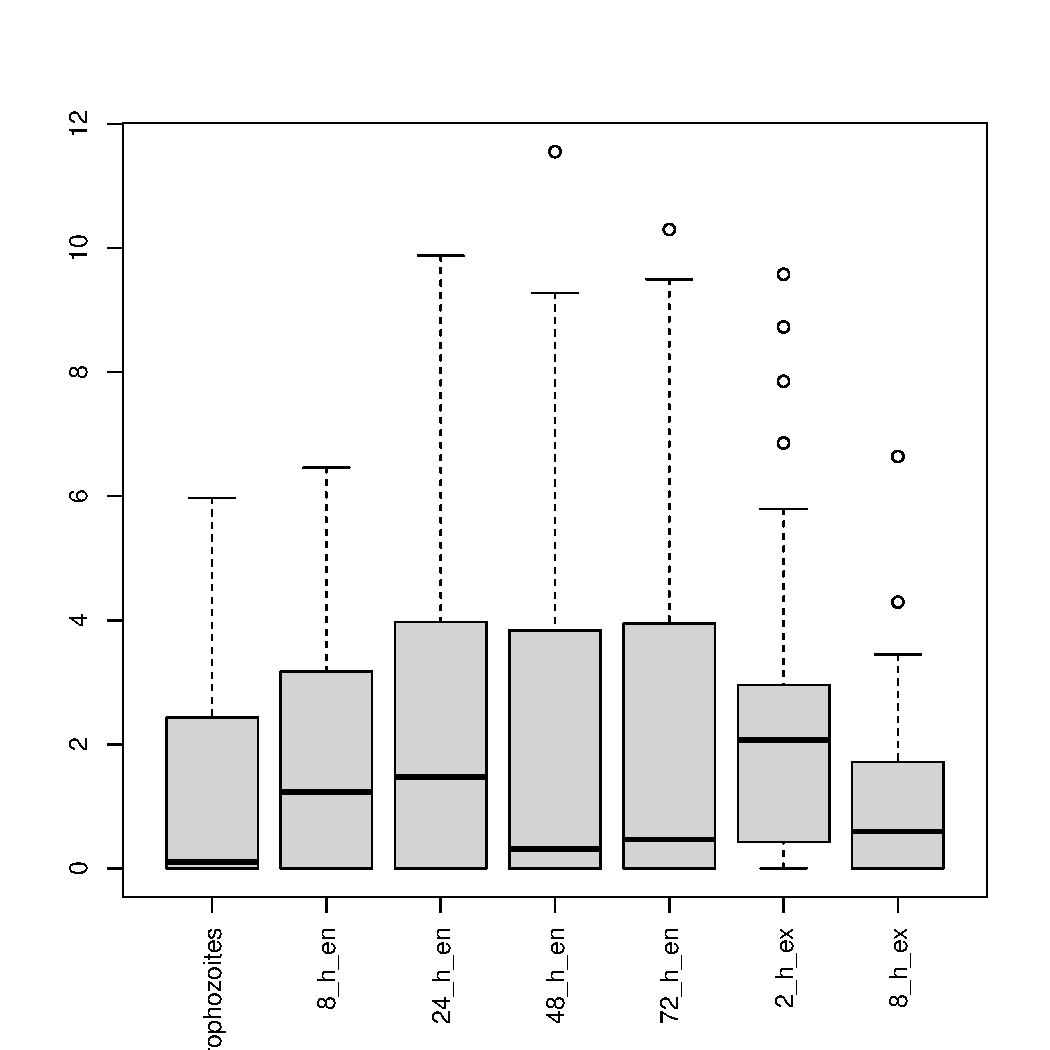
\includegraphics[width=0.8\textwidth]{BoxPlotDatosTransformadosLog2.pdf}
  \caption{Box-plot de los datos despues de aplicarles $Log_{2}$.}
  \label{fig:heatmap_example}
\end{figure}





\end{document}